\documentclass[10pt]{article}
\usepackage[margin=2cm]{geometry}
\setlength{\parskip}{0.5em}
\setlength\parindent{0pt}
\interfootnotelinepenalty=10000

% % Language and font encodings
% \usepackage[english]{babel}
% \usepackage[utf8x]{inputenc}
% \usepackage[T1]{fontenc}

\usepackage{amssymb}
\usepackage{amsmath}

% figures and tables
\usepackage{graphicx}
% \graphicspath{{data/}}
\usepackage{subfigure}	
\usepackage{float}
\usepackage{chemformula}		
\setlength{\floatsep}{10pt plus 2.0pt minus 2.0pt}
\usepackage{caption}
% \usepackage{pdfpages}
% \usepackage{epstopdf}
% \usepackage{svg}
% \usepackage{pgfplots}
% \pgfplotsset{compat=newest}
\setlength\tabcolsep{1em}
\usepackage{multirow}
\renewcommand{\arraystretch}{1.3}

\usepackage[font=footnotesize,labelfont=bf]{caption}

% science
\usepackage{siunitx}
\DeclareSIUnit{\molar}{M}
\usepackage{chemformula}

% miscellaneous 
\usepackage{enumitem}	
\usepackage{verbatim}
\usepackage{xcolor}
\usepackage[color=cyan]{todonotes}
\usepackage[colorlinks=true, allcolors=blue]{hyperref}
\usepackage[sort,comma,numbers]{natbib}
\bibliographystyle{plainnat}

\renewcommand{\abstractname}{\vspace{-\baselineskip}}

\newcommand{\note}[1]{\colorbox{cyan}{#1}}

\title{\vspace{-2cm} \textsc{\underline{Laboratory Report \#11}} \\ \textbf{Travelling Salesman Problem: the Quasi-Optimal Chemotactic Renormalisation Solution} \vspace{-0.5cm}}
\author{\textsc{Benjamin Huang and Shiye Su}}
\date{}

\begin{document}
\maketitle

\begin{abstract}

Using the chemotaxis of \textit{C. elegans} worms on a biased \ch{NaCl} gradient, we develop and extend the method of renormalisation groups discussed by \citet{Yoshiyuki1995} to find a quasi-optimal solution to the Traveling Salesman Problem (TSP). The trajectories of worms grown at \SI{50}{\milli\molar} \ch{NaCl} moving on a \SI{50}{\milli\molar} plate with \SI{200}{\milli\molar} cities are tracked. The convergences of trajectory radii of a worm leaving each city are processed into a traversal path--a quasi-optimal solution to the TSP. Our results show that for our small city configuration this method of \emph{chemotactic renormalisation} yields the optimal path length for more than 80\% of trials. Both the mean chemotactic and gridding renormalisation improve upon the length of a randomly selected path by more than 15\%. However, chemotaxis achieved 1\% deviation from optimal contrasted to gridding's 7\%. Our results are promising, as TSP is a NP-complete problem of great theoretical interest and broad applications; our results should motivate further study in organically-inspired, stochastic heuristics for optimization problems.

\end{abstract}

\section{Introduction}

The traveling salesperson problem (TSP) is a classic problem in combinatorial optimization. The problem asks to find the shortest route that visits $n$ cities exactly once, except for the first and last cities, which are the same. As an NP-complete problem that is $O(n!)$, exact algorithms have not improved beyond worst-case $O(n^22^n)$, which is costly in time and computing resources \citep{Held1962}. An active field of research focuses on heuristics and approximate solutions, including greedy algorithms, simulated annealing, and renormalization, where balancing computation time and solution accuracy are paramount. TSP has broad applications in operations research, circuit design, materials fabrication, and DNA sequencing, and is related to problems of theoretical significance in graph theory.

\par Renormalization theory, in essence, concerns a \textit{rescaling} of a problem. As used by \citet{Yoshiyuki1995}, the TSP can be simplified by ``zooming out;'' a map of cities, seen from far away, will appear to only have a few clusters of cities. Since exact TSP algorithms are $O(n^22^n)$, a problem with a small number of cities ($n \approx 4$) is trivial to solve. Figure \ref{fig:grid} shows how this concept was applied by \citet{Yoshiyuki1995} to reduce the TSP into a large number of smaller problems, iteratively solving for smaller and smaller clusters of cities, until clusters are single cities. This is done through what we will call \emph{orthogonal gridding}, which recursively divides the cities into four quadrants. \citet{Yoshiyuki1995} found a tour 30\% longer than the optimal tour for a 532 US city problem.

\begin{figure}[H]
  \centering
  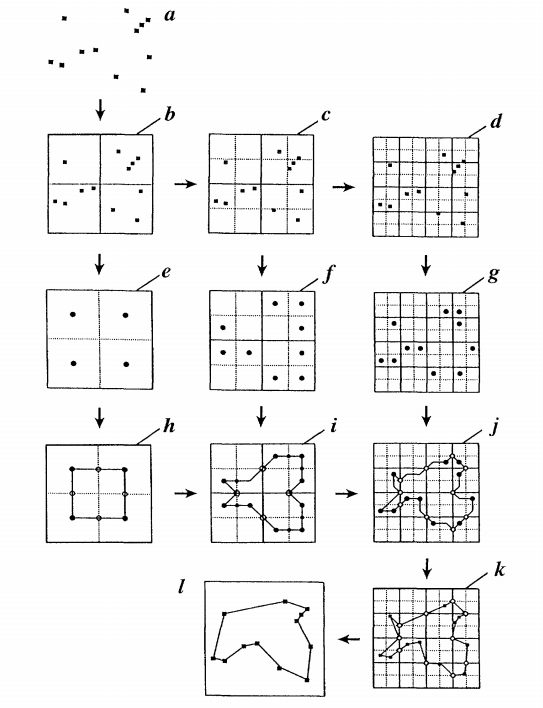
\includegraphics[height = 5.5cm, trim={0 0 0 2.85cm}, clip]{figUsami}
  \caption{Renormalization process presented by \citet{Yoshiyuki1995}. Subdivisions increase towards the right,
    increasing the number of 4-city problems to solve. These solutions are combined with larger solutions 
    (fatherst left column) to connect all of them.}
  \label{fig:grid}
\end{figure}

\par Other methods besides orthogonal gridding have been explored to extend upon the work of \citet{Yoshiyuki1995}. \citet{Ugajin2002} employed the inverse diffusion process to cluster cities based on a reverse diffusion process. He grouped cities by the convergence of diffusing point sources, where each point source was a city. Two cities were said to have \emph{converged} when the edges of the diffusing material mixed. His results show an improvement over \citet{Yoshiyuki1995} on the 532 US city problem to 17\% longer than optimal. Furthermore, renormalization theory has been extended in optimization problems in combination with genetic algorithms by \citet{Houdayer1999}. Their results show a genetic-renormalization algorithms ability to achieve optimal or very close to optimal (at worst, 0.0056 \% longer) solutions in a fraction of the computation time.

\par Optimization problems have been solved using organically-inspired solutions (such as ant colony optimization), but never have they been used in conjunction with renormalization theory.
Building off of the work of \citet{Yoshiyuki1995} and \citet{Ugajin2002}, we investigate  
a new, probabilistic way of clustering cities based on the chemotaxis of \textit{Caenorhabditis 
elegans} (\textit{C. elegans}). The chemotaxis of \textit{C. elegans} in response to \ch{NaCl} is well documented as an intricate phenomenon, leading to our interest in their ability to cluster cities effectively for renormalization.

\section{Materials and Methods}

\textit{C. elegans} worms were grown at \SI{50}{\milli\molar} \ch{NaCl}. Agar plates were made at
\SI{50}{\milli\molar} \ch{NaCl}. Using a plate-sized template of a six-city configuration labelled A-F (see
Figure \ref{figsol}), a \SI{5}{\micro\litre} solution of \SI{200}{\milli\molar} \ch{NaCl} was spotted on the
surface of the agar at each city location. The salt solution was allowed to diffuse into and through the agar for
$\approx \SI{30}{\minute}$. The time to diffuse was estimated using code written by Andrew Leifer, which was 
based on Fick's equations and Neumann boundary conditions. One \textit{C. elegans} worm was placed at one city.
Immediately afterwards, the plate was placed inside a ring light and the mounted camera commenced image sequence
acquisition for 5 minutes at 2 frames per second (600 frames). Using a new worm and new plate, this imaging
process was repeated 4-5 times for each city. The $x$-$y$ coordinates of each worm's trajectory was extracted
via image processing for analysis.

\par A set of six worms, one from each city, was chosen and each's trajectory converted into a displacement from
its starting position. Figure \ref{figchem} shows our procedure for chemotaxis clustering: overlapping
displacements are \emph{convergences}. To convert convergences into a tour, pairs of converging cities are
merged into \emph{groups}. If a city merges with another city already in a group, the city is added to whichever
end it is closer to. When two groups are merged, all ends are compared against each other (4 comparisons). Groups
were then merged with the two cities with the shortest distance being in the middle. Groups were not allowed to
be interuppted. See Appendex for an example of this merging process. In summary, our computation processes
chemotactic trajectories into a city convergence order, into a final path. To produce a large number of results,
we used every permutation of trial possible. 4 trials from each city were used, producing $4^6$ possible routes.
Refer to appended script for implementation details.

\begin{figure}[H]
	\centering
	\subfigure[]{\includegraphics[width=0.3\textwidth, trim={5cm 8cm 5cm 8cm}, clip]{figchem1.pdf}}
	\subfigure[]{\includegraphics[width=0.3\textwidth, trim={5cm 8cm 5cm 8cm}, clip]{figchem2.pdf}}
	\subfigure[]{\includegraphics[width=0.3\textwidth, trim={5cm 8cm 5cm 8cm}, clip]{figchem3.pdf}}
	\caption{Chemotaxis renormalisation procedure, shown for one arbitrarily chosen set of  worms leaving each city. In this set, cities C and D are the first to converge (a), then A and C, then F and C (b). All cities have converged (homogenized) by Frame 300 (c).}
	\label{figchem}
\end{figure}


\section{Results and Discussion}

Figure \ref{figdye} provides evidence that our spotting method indeed creates a radial gradient. Methylene blue dye, with mass \SI{319.85}{\gram\per\mol} and size \SI{10}{\angstrom} was used for visualisation. \ch{Na} and \ch{Cl} ions, of mass and size an order of magnitude smaller, are expected to have diffusion coefficient an order of magnitude greater. As discussed in methods, the appropriate time to establish the desired gradient is \SI{30}{\min}.

The rationale for such an experimental setup is that via chemotaxis, \textit{C. elegans} worms seek the environment in which they were grown, in this case an ambient \SI{50}{\milli \molar} \ch{NaCl} concentration. Thus, in theory they are motivated away from the concentrated \ch{NaCl} city locations at a rate positively correlated to the concentration at the cities. The plate has higher \ch{NaCl} concentration for regions of high city density; the worms chemotaxis away from these cities more rapidly, resulting in an earlier convergence of these cities. Intuitively, this is sound for TSP as geographically close cities should be traversed in succession.

Furthermore, we think the probabilistic nature of chemotaxis culd be beneficial to a TSP algorithm. Because the worms' trajectories are non-deterministic, renormalisation with chemotaxis facillitates exploration of more routes in the sample space, potentially finding a better solution. This contrasts diffusion, which being essentially deterministic, would consistently yield a form of `greedy' nearest-distance grouping. 

\begin{figure}[H]
	\centering
	\subfigure[Before]{\includegraphics[width=0.25\textwidth]{figbefore.png}}
	\subfigure[After]{\includegraphics[width=0.25\textwidth]{figafter.png}}
	\caption{Methylene blue dye spotted on agar surface using the method described above, allowed to diffuse 
          for 12 hours.}
	\label{figdye}
\end{figure}

We present our solutions to this particular city configuration in Figure \ref{figsol}. Orthogonal gridding (a) divides the configuration into quadrants containing D, A, B, and F, C, and A respectively. A second division of the latter quadrant separates F, C, and A; using the method presented by \citet{Yoshiyuki1995}, the appropriate path is CFE. This yields the solution ABEFCDA, with a path length of \SI{0.1034}{\metre} and a 7\% deviation from optimal, as seen in Table \ref{tab}. Chemotactic renormalisation, as we illustrated in Figure \ref{figchem}, considers the convergences of radiis of worm trajectories. This yielded the solution ABEFCDA, the optimal solution to the TSP.

We noted that orthogonal gridding is arbitrary in its division of the map into quadrants. Furthermore, we see that this division is sensitive to the framing of the map, so that the absolute rather than relative coordinates of the city become important in the renormalisation solution. Conversely, the chemotactic renormalisation deals with relative distances, an advantage over gridding.

As shown in Table \ref{tab} and Figure \ref{fighist}, the chemotactic process overwhelmingly produced the optimal solution to this TSP. The median and mode chemotactic path lengths coinciding exactly with the optimal path length, and mean chemotactic path length was longer by less than 1\%. This reflected in Figure \ref{fighist}. The distribution of chemotactic solutions heavily favours the optimal \SI{0.0965}{\metre}, with a few longer path solutions. Both chemotaxis and gridding have a substantial percent improvement upon some randomly chosen path (likely even greater for a less symmetrically clustered configurations), and the distribution supports that the chemotactic solution is at least on average no worse than gridding.


\begin{figure}[H]
	\centering
    \subfigure[Solution: ABEFCDA]{\includegraphics[width=0.4\textwidth, trim={2cm 8cm 2cm 8cm},clip]{figgrid.pdf}}
    \subfigure[Solution: ABEFDCA]{\includegraphics[width=0.4\textwidth, trim={2cm 8cm 2cm 8cm},clip]{figchem.pdf}}
    \caption{Renormalisation (orthogonal and chemotactic) solutions. The solution to this TSP, found with computational brute force (refer to appendix for script) is ABEFDCA, which is the solution overwhelmingly found via chemotaxis (Refer to Figure \ref{fighist}). Gridding algorithm, as it is deterministic, was excuted once. The chemotactic renormalization was the median solution from $4^6$ separate sets of worm trajectories.}
    \label{figsol}
\end{figure}

\begin{table}[H]
	\centering
	\begin{tabular}{c | c c c}
	\hline
	\textsc{Method} & \textsc{Distance} (\SI{}{\meter}) & \textsc{Percent Improvement} & \textsc{Deviation from Optimal} \\
	\hline
	Optimal 					& 0.0965 & 22.3\% & 0\% 	\\
    Median and mode chemotactic & 0.0965 & 22.3\% & 0\% 	\\
	Mean chemotactic 			& 0.0973 & 21.2\% & .88\% 	\\
    Worst chemotactic 			& 0.1200 & 3.3\%  & 24.4\% 	\\
	Orthogonal gridding 		& 0.1034 & 16.7\% & 7.2\% 	\\
	\hline
	\end{tabular}
	\caption{Path distances, percent improvement from the median path length of all possible traversals (calculated as $ \frac{\text{median} - \text{this path}}{\text{median}} $), and percent deviation from the path length of the optimal solution of this TSP (calculated as $ \frac{\text{this path} - \text{optimal}}{\text{optimal}} $). We do not include error here because the coordinates of the cities are without uncertainty by construction.}
	\label{tab}
\end{table}


\begin{figure}[H]
	\centering
    \includegraphics[width=0.7\textwidth, trim={0 8cm 0 9cm}, clip]{fighist.pdf}
    \caption{Probability distribution of path distances for all possible traversals of the configuration, all chemotatically renormalised paths, and orthogonal gridding. The solution path length is \SI{0.0965}{\metre} (contained in leftmost chemotactic bin). ''All Possible Paths'' are every single possible path ($\frac{5!}{2}$). ''Chemotactic Paths'' are from $4^6$ separate sets of worm trajectories. Orthogonal gridding was performed only once.}
    \label{fighist}
\end{figure}

In our experiment, the measurement errors of the worms' exact positions are relatively insignificant to our calculations of the solution. It is important, however, that all image sequences are correctly calibrated, as this is likely to affect the order or convergences and thus the final solution. There is `error' in the sense that worm trajectories are stochastic - a property of chemotaxis we wanted to explore. For futher investigation, we would quantify and evaluate the mean squared displacements and standard deviations of worms leaving each city.

Lastly, we acknowledge that our city configuration is small and solvable by inspection. Our findings are based on one configuration, and we concede that more configurations including `corner cases' should be explored to properly assess this method's power. Nevertheless, our results suggest that chemotactic renormalisation is in principle sound. If the experiment were extended to larger configurations, we expect the differences in gridding and chemotactic solutions to be widened, and the distribution of chemotactic path lengths (Figure \ref{fighist}) to be more widely spread but remain positively skewed.


\section{Conclusion}

Our results illustrate the potential advantages of chemotactic renormalization over orthogonal gridding. More than 80\% of our chemotactic solutions coincided with the optimal solution ABEFDCA, with a path length of \SI{0.0965}{\metre} and improvement of more than 20\% from the median of all possible path lengths. This is a substantial improvement over the rudimentary arbitrary gridding technique outlined by \citet{Yoshiyuki1995}, which deviates from optimal by 7\% for our city arrangement. 

These findings confirm our expectations that a chemotactic heuristic sensitive to the city configuration improves upon gridding. Future research could investigate other natural phenomenon that are viable renormalisation techniques, and ultimately characterize these systems to produce a computational heuristic for TSP, which combines the merits of nearest-distance (chemotaxis is similar to diffusion) and stochastic algorithms like simulated annealing (chemotaxis is nondeterministic). We would be interested to compare the results and runtime of an algorithm with greedy, gridding, and simulated annealing algorithms. As we discussed, there are extensive applications to operations optimization, manufacture, and genomics.


\section{Acknowledgements}

We sincerely thank Dr. Jennifer Gadd, Dr. Quan Wang, Mochi Liu, and Sagar Setru for laboratory assistance and helpful suggestions to our experimental method. Thank you especially to Dr. Gadd for accommodating our requests. Thanks also goes to Dr. Andrew Leifer of Princeton University for the script that estimates rate of diffusion of salt in agar. Thank you the ISC class for valuable feedback in our experimental proposal and moral support. In particular, we are grateful to Chris Russo for harsh criticism and mockery; to Henry Ando for believing in the computational power of \textit{C. elegans}; to Alice Lin for giving us a paper on Monte Carlos Markov Chains and subsequently making us obsessed with them; and to Austin (Han Jie) Wang and Olivia Long for providing the worst soundtrack of pure tones ever to do our work to. Finally, we are indebted to our \text{C. elegans}, who showed that P=NP.

\bigskip
\begin{center}
\textbf{This paper represents our own work in accordance with University regulations}\\ -- Shiye Su \& Benjamin Huang
\end{center}

\clearpage
\bibliography{Lab11}

\section{Supplementary Information}

\subsection{Appendix}

\textbf{Example of our merging algorithm:} Let cities A and B (neither in groups) converge. Then, they form a 
group \{A, B\}. Let C converge with A, where C is in the group \{C, D, E, F\}. The resultant ordered group is
either \{A,~B,~C,~D,~E,~F\}, \{B, A, C, D, E, F\}, \{C, D, E, F, A, B\}, or \{C, D, E, F, B, A\}, depending on
the concatenation that yields the smallest distance between the connecting cities. The ordering of each group 
must be preserved or completely reversed in concatenating new group (insertions into the center of a group were
not allowed).


\subsection{MATLAB Code}

\begin{verbatim}
% Motivation: http://www.wormbook.org/wbg/articles/volume-18-number-3/making-linear-chemical-gradients-in-agar/
%
% Question: how many days before can we get away with?
%
%Fick's equation is
%
% dc/dt =D d^2 C/ dx^2 where the d's are partials
%
% Since the petri dish is a solid boundary, we have neumann boundary conditions
%
%
%
% Created by Dr. Andrew Leifer
%
% From resources like:
% http://ramanujan.math.trinity.edu/rdaileda/teach/s12/m3357/lectures/lecture_2_28_short.pdf
%
% http://texas.math.ttu.edu/~gilliam/fall03/m4354_f03/heat_N_web/heat_ex_homo_neum.pdf
%
% we know the general solution
%
%
% for the specific initial conditions f(x)=x*C0 / L,
%
% I figure that we only really care about x=0 because if we know u(x=0,t) we
% should know that u(x=L,t)=C0 - u(x=0,t).
%
% And I assume that the profile along x is roughly linear, although we could check.
 
 
 
 
 
L=1;%cm - width of the petri dish
C0=200; %mM - highest concentration assuming lowest concentration is 0mM
D=0.84*10^-5; %cm^2 / s - diffusion coefficient of solute
days=0.12; %number of days the plates will be allowed to equilibrate
 
 
 
disp('Calculating the concentration at the far end of the plate x=0.');
disp(['We assume a ' num2str(L) 'cm plate with an initial concentration gradient from 0 to ' num2str(C0) ' mM  and D=' num2str(D) 'cm^2/s' ]);
t=0:3*60*60*24*7; %3 weeks
u=C0/2;
for n=1:2:1000
    u= u + ( 2*C0/(pi^2) )*(-2/(n^2))*exp(-D* t*(n*pi/L)^2  );
  end
figure; plot(t/(60*60*24),u);
xlabel('Days')
ylabel('Concentration at x=0 (mM)') %concentration at the end initially with concentration of 0mM
title('Concentration of Solute Based on Equilibration Time')

 
disp(['After ' num2str(days) ...
    'days the concentrations at the end point will be '...
    num2str( u(round(days*60*60*24)) )  'mM and ' ...
    num2str(C0-u(round(days*60*60*24)) ) 'mM'] )


path = 'C:\Users\bdhua\Documents\Schoolwork\2017_S\ISC233\Laboratories\Lab11\Tracks\Tracks';
cd(path);

d = dir('*.txt');
fnames = {d.name}';
Ntrials = length(fnames);
[A,B,C,D,E,F] = deal(cell(1,1));

for i=1:Ntrials
    data = importdata(fnames{i});
    switch fnames{i}(1)
        case 'A'
            A = vertcat(A,{data.data});
        case 'B'
            B = vertcat(B,{data.data});
        case 'C'
            C = vertcat(C,{data.data});
        case 'D'
            D = vertcat(D,{data.data});
        case 'E'
            E = vertcat(E,{data.data});
        case 'F'
            F = vertcat(F,{data.data});
    end
end
A = A(2:end);
B = B(2:end);
C = C(2:end);
D = D(2:end);
E = E(2:end);
F = F(2:end);

Arad = calcRadius(A);
Brad = calcRadius(B);
Crad = calcRadius(C);
Drad = calcRadius(D);
Erad = calcRadius(E);
Frad = calcRadius(F);
rads = {Arad,Brad,Crad,Drad,Erad,Frad};

%% Cities

% import configuration
cities = importdata('cities.txt');
c_names = cell2mat(cities.rowheaders);
c_coord = cities.data / 100;
nCities = length(c_names);
%% Get city distances

c_dists = zeros(size(c_names,1),size(c_names,1));
for i=1:size(c_names,1)
    for j=(i+1):size(c_names,1)
        c_dists(i,j) = sqrt((c_coord(i,1) - c_coord(j,1))^2 + ...
            (c_coord(i,2) - c_coord(j,2))^2);
    end
end

c_dists = reshape(transpose(c_dists), 1, []);
c_dists = c_dists(c_dists~=0); % ith entry is distance between cities given by labels{i}

%% Combinatorics of trials per city

combs = combntns([1 1 1 1 1 1 2 2 2 2 2 2 3 3 3 3 3 3 4 4 4 4 4 4], 6);
combs = unique(combs, 'rows');
permuts = int16.empty;
for i=1:size(combs,1)
    compare = perms(combs(i,:));
    permuts = unique(vertcat(permuts, compare), 'rows');
end
clear temp; clear i

%% results for one set of results for one worm from each city

pairs = combntns(1:nCities,2); % possible pairings of two cities
nPairs = size(pairs,1);

combos = {};
for i=1:size(permuts,1) 
    combos{i} = double.empty;
    for j=1:nPairs % each combination of two pairs
        ind1 = pairs(j,1);
        ind2 = pairs(j,2);
        compare = rads{ind1}(:, permuts(i,ind1)) ...
            + rads{ind2}(:, permuts(i,ind2));
        combos{i} = horzcat(combos{i}, compare);
    end
end
clear ind1; clear ind2;

labels = {}; % nth entry is the 
for i=1:nPairs
    labels{i} = strcat(c_names(pairs(i,1)), c_names(pairs(i,2))); % use char references
    % labels{i} = [pairs(i,1), pairs(i,2)]; % use int references
end

%% Find order of convergence

converge = {};
twoConverge = {};
for i=1:size(combos,2)
    compare = combos{i} > c_dists;
    converge{i} = NaN(1, nPairs);
    for j=1:size(compare, 2)
        [row, col] = find(compare);
        try
            converge{i}(j) = min(row(col == j));
        catch
        end
    end
    nNotNans = sum(~isnan(converge{i}));
    [~, temp] = sort(converge{i}); % order in which two cities converge
    twoConverge{i} = temp(1, 1:nNotNans);
end
clear row; clear col; clear compare;

%% Find quasi-optimal path
paths = cellfun(@(x) groupCity(x,c_dists),twoConverge,'UniformOutput',false);
pthdists = cellfun(@(x) nansum(c_dists(ismember(pairs,sort([x',[x(2:end)';...
    x(1)]],2),'rows'))),paths);
% Remove nan values
pthdists = pthdists(pthdists > 0);

%% BRUTE FORCE SOLUTION %%
% this really could be optimised a lot

routes = perms([1:nCities]);
dist = zeros(length(routes),1);
for k=1:length(routes)
    dist(k) = sum(c_dists(ismember(pairs,...
    sort([routes(k,:);[routes(k,2:end),routes(k,1)]])','rows')));
end

[optPathDist, index] = min(dist);
wrsPathDist = max(dist);
avgPathDist = median(dist);
optPathInt = routes(index, :);
optPathStr = '';
for i=1:nCities
    optPathStr = strcat(optPathStr, c_names(optPathInt(i)));
end

%% Gridded result
gridr = [5,6,3,4,1,2];
gridd = sum(c_dists(ismember(pairs,...
    sort([gridr;[gridr(2:end),gridr(1)]]',2),'rows')));

%% Another look at radius/city:
avgrads = cellfun(@(x) mean(x,2),rads,'UniformOutput',false);
stdrads = cellfun(@(x) std(x,1,2),rads,'UniformOutput',false);
[stdfilx,stdfily] = cellfun(@(x,y) errEnvelop(0:.5:299.5,y,x),stdrads,...
    avgrads,'UniformOutput',false);
stdfilx = [stdfilx{:}]; stdfily = [stdfily{:}];
avgrads = [avgrads{:}];

% Figures
cols = linspecer(6);
figure(1); clf;
axis tight; grid on;
subplot(2,1,1); hold on;
p = plot(0:.5:299.5,avgrads);
f = fill(stdfilx,stdfily,'k');
for i=1:length(f)
    f(i).FaceAlpha = .2;
    f(i).LineStyle = 'none';
    f(i).FaceColor = cols(i,:);
    p(i).Color = cols(i,:);
end
subplot(2,1,2)
plot(0:.5:299,movmean(diff(avgrads)/.5,50));

%% Figure aesthetics!
figure(2); clf;
axis tight; hold on; grid minor; grid on;
h1 = histogram(unique(dist),10,'normalization','probability');
h2 = histogram(pthdists,10,'normalization','probability');
ylim([0 1]);
gr = line([gridd gridd],ylim);
gr.LineStyle = '--'; gr.Color = 'k';
legend([h1 h2 gr],{'All Possible Paths','Chemotactic Paths',...
    ['Orthogonal',char(10),'Gridding Path']},'FontSize',12);
xlabel('Path Distance (m)'); ylabel('Probability (a.u.)');


path = 'C:\Users\bdhua\Documents\Schoolwork\2017_S\ISC233\Laboratories\Lab11\Tracks\Tracks';
cd(path);

d = dir('*.txt');
fnames = {d.name}';
Ntrials = length(fnames);
[A,B,C,D,E,F] = deal(cell(1,1));

for i=1:Ntrials
    data = importdata(fnames{i});
    switch fnames{i}(1)
        case 'A'
            A = vertcat(A,{data.data});
        case 'B'
            B = vertcat(B,{data.data});
        case 'C'
            C = vertcat(C,{data.data});
        case 'D'
            D = vertcat(D,{data.data});
        case 'E'
            E = vertcat(E,{data.data});
        case 'F'
            F = vertcat(F,{data.data});
    end
end
A = A(2:end);
B = B(2:end);
C = C(2:end);
D = D(2:end);
E = E(2:end);
F = F(2:end);

Arad = calcRadius(A);
Brad = calcRadius(B);
Crad = calcRadius(C);
Drad = calcRadius(D);
Erad = calcRadius(E);
Frad = calcRadius(F);
rads = {Arad,Brad,Crad,Drad,Erad,Frad};

%% Cities

% import configuration
cities = importdata('cities.txt');
c_names = cell2mat(cities.rowheaders);
c_coord = cities.data / 100;
nCities = length(c_names);
%% Get city distances

c_dists = zeros(size(c_names,1),size(c_names,1));
for i=1:size(c_names,1)
    for j=(i+1):size(c_names,1)
        c_dists(i,j) = sqrt((c_coord(i,1) - c_coord(j,1))^2 + ...
            (c_coord(i,2) - c_coord(j,2))^2);
    end
end

c_dists = reshape(transpose(c_dists), 1, []);
c_dists = c_dists(c_dists~=0); % ith entry is distance between cities given by labels{i}

%% Combinatorics of trials per city

combs = combntns([1 1 1 1 1 1 2 2 2 2 2 2 3 3 3 3 3 3 4 4 4 4 4 4], 6);
combs = unique(combs, 'rows');
permuts = int16.empty;
for i=1:size(combs,1)
    compare = perms(combs(i,:));
    permuts = unique(vertcat(permuts, compare), 'rows');
end
clear temp; clear i

%% results for one set of results for one worm from each city

pairs = combntns(1:nCities,2); % possible pairings of two cities
nPairs = size(pairs,1);

combos = {};
for i=1:size(permuts,1) 
    combos{i} = double.empty;
    for j=1:nPairs % each combination of two pairs
        ind1 = pairs(j,1);
        ind2 = pairs(j,2);
        compare = rads{ind1}(:, permuts(i,ind1)) ...
            + rads{ind2}(:, permuts(i,ind2));
        combos{i} = horzcat(combos{i}, compare);
    end
end
clear ind1; clear ind2;

labels = {}; % nth entry is the 
for i=1:nPairs
    labels{i} = strcat(c_names(pairs(i,1)), c_names(pairs(i,2))); % use char references
    % labels{i} = [pairs(i,1), pairs(i,2)]; % use int references
end

%% Find order of convergence

converge = {};
twoConverge = {};
for i=1:size(combos,2)
    compare = combos{i} > c_dists;
    converge{i} = NaN(1, nPairs);
    for j=1:size(compare, 2)
        [row, col] = find(compare);
        try
            converge{i}(j) = min(row(col == j));
        catch
        end
    end
    nNotNans = sum(~isnan(converge{i}));
    [~, temp] = sort(converge{i}); % order in which two cities converge
    twoConverge{i} = temp(1, 1:nNotNans);
end
clear row; clear col; clear compare;

%% Find quasi-optimal path
paths = cellfun(@(x) groupCity(x,c_dists),twoConverge,'UniformOutput',false);
pthdists = cellfun(@(x) nansum(c_dists(ismember(pairs,sort([x',[x(2:end)';...
    x(1)]],2),'rows'))),paths);
% Remove nan values
pthdists = pthdists(pthdists > 0);

%% BRUTE FORCE SOLUTION %%
% this really could be optimised a lot

routes = perms([1:nCities]);
dist = zeros(length(routes),1);
for k=1:length(routes)
    dist(k) = sum(c_dists(ismember(pairs,...
    sort([routes(k,:);[routes(k,2:end),routes(k,1)]])','rows')));
end

[optPathDist, index] = min(dist);
wrsPathDist = max(dist);
avgPathDist = median(dist);
optPathInt = routes(index, :);
optPathStr = '';
for i=1:nCities
    optPathStr = strcat(optPathStr, c_names(optPathInt(i)));
end

%% Gridded result
gridr = [5,6,3,4,1,2];
gridd = sum(c_dists(ismember(pairs,...
    sort([gridr;[gridr(2:end),gridr(1)]]',2),'rows')));

%% Another look at radius/city:
avgrads = cellfun(@(x) mean(x,2),rads,'UniformOutput',false);
stdrads = cellfun(@(x) std(x,1,2),rads,'UniformOutput',false);
[stdfilx,stdfily] = cellfun(@(x,y) errEnvelop(0:.5:299.5,y,x),stdrads,...
    avgrads,'UniformOutput',false);
stdfilx = [stdfilx{:}]; stdfily = [stdfily{:}];
avgrads = [avgrads{:}];

% Figures
cols = linspecer(6);
figure(1); clf;
axis tight; grid on;
subplot(2,1,1); hold on;
p = plot(0:.5:299.5,avgrads);
f = fill(stdfilx,stdfily,'k');
for i=1:length(f)
    f(i).FaceAlpha = .2;
    f(i).LineStyle = 'none';
    f(i).FaceColor = cols(i,:);
    p(i).Color = cols(i,:);
end
subplot(2,1,2)
plot(0:.5:299,movmean(diff(avgrads)/.5,50));

%% Figure aesthetics!
figure(2); clf;
axis tight; hold on; grid minor; grid on;
h1 = histogram(unique(dist),10,'normalization','probability');
h2 = histogram(pthdists,10,'normalization','probability');
ylim([0 1]);
gr = line([gridd gridd],ylim);
gr.LineStyle = '--'; gr.Color = 'k';
legend([h1 h2 gr],{'All Possible Paths','Chemotactic Paths',...
    ['Orthogonal',char(10),'Gridding Path']},'FontSize',12);
xlabel('Path Distance (m)'); ylabel('Probability (a.u.)');



\end{verbatim}

\end{document}